\documentclass[conference]{IEEEtran}
\IEEEoverridecommandlockouts
% The preceding line is only needed to identify funding in the first footnote. If that is unneeded, please comment it out.
\usepackage{cite}
\usepackage{amsmath,amssymb,amsfonts}
\usepackage{algorithmic}
\usepackage{graphicx}
\usepackage{listings}
\usepackage{textcomp}
\usepackage{xcolor}
\def\BibTeX{{\rm B\kern-.05em{\sc i\kern-.025em b}\kern-.08em
    T\kern-.1667em\lower.7ex\hbox{E}\kern-.125emX}}
\begin{document}

\title{Conference Paper Title}

\author{\IEEEauthorblockN{Taylor Abraham}
\IEEEauthorblockA{\textit{Systems and Computer Engineering} \\
\textit{Carleton University}\\
Ottawa, Canada \\
email address or ORCID}
\and
\IEEEauthorblockN{David Bascelli}
\IEEEauthorblockA{\textit{Systems and Computer Engineering} \\
	\textit{Carleton University}\\
	Ottawa, Canada \\
	email address or ORCID}
\and
\IEEEauthorblockN{Joshua Fryer}
\IEEEauthorblockA{\textit{Systems and Computer Engineering} \\
	\textit{Carleton University}\\
	Ottawa, Canada \\
	joshfryer@cmail.carleton.ca}
\and
\IEEEauthorblockN{Zein Hajj-Ali}
\IEEEauthorblockA{\textit{Systems and Computer Engineering} \\
	\textit{Carleton University}\\
	Ottawa, Canada \\
	email address or ORCID}
}

\maketitle

\begin{abstract}
A team of Robocup soccer-playing agents was implemented using the Jason framework\footnote{http://jason.sourceforge.net/wp/}, creating a team of five Jason agents which communicate with each other and execute plans; these agents perceived and acted upon the virtual soccer field by interfacing with Krislet entities. The team demonstrated cooperative behaviour in scoring on the opposing net and preventing scoring on the friendly net.
\end{abstract}

\section{Introduction}
Our goal was to design and implement a multi-agent system of agents that communicated and exhibit coordination to (reasonably) successfully play soccer in the Robocup soccer simulation. Jason was chosen as the framework because it extends the already-useful AgentSpeak language’s basis for belief-desire-intention (BDI) programming with inter-agent communication and a shared abstract environment to help manage the agents’ percepts and execute their actions. 

\section{Design}

\subsection{BDI Architecture}
Our agents use a Belief-Desire-Intention (BDI) design; they hold beliefs (things they know about the world and themselves, such as their position relative to objects, or messages they have been given by other agents), desires or goals (a collection of beliefs they wish to hold and maintain, such as having kicked the ball towards the opposing net), and intentions or plans to reach those goals given their current set of beliefs. 
\begin{figure}[h]
	\centering
	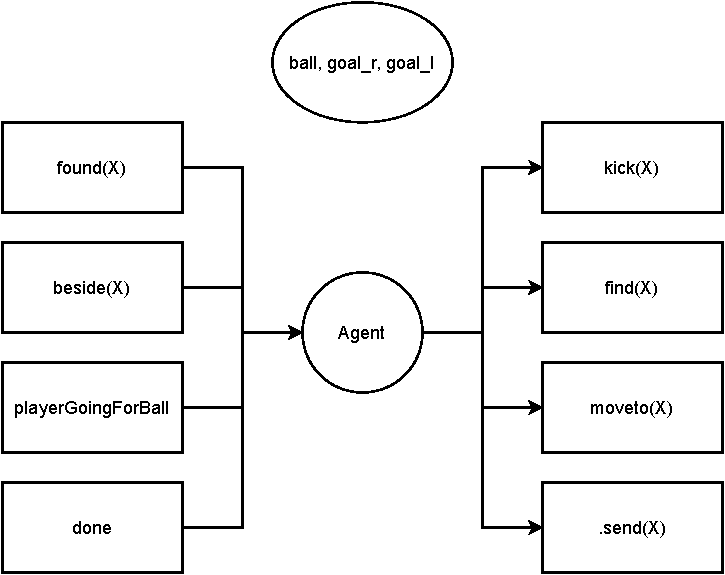
\includegraphics[scale=0.5]{fig/percepts-and-actions.pdf}
	\caption{Some key percepts and actions used in our agents}
	\label{percepts-actions}
\end{figure}


\subsection{Goals and Planning}

We designed two types of player agent, to fulfill different roles: offensive players ("strikers"), and defensive players ("defenders"). Their decision processes are as follows:

\subsubsection{Strikers}
The first striker to see the ball will take on the role of primary attacker, and will attempt to kick the ball into the net. It notifies the other strikers of this, and they take on an assisting role and run towards the opposing net. When the attacking striker kicks, it notifies all strikers and the distance calculation and role assignment happens again. Figure \ref{sequence-diagram} is a sequence diagram illustrating the interplay and communication of the striker agents 
\begin{figure}[]
	\centering
	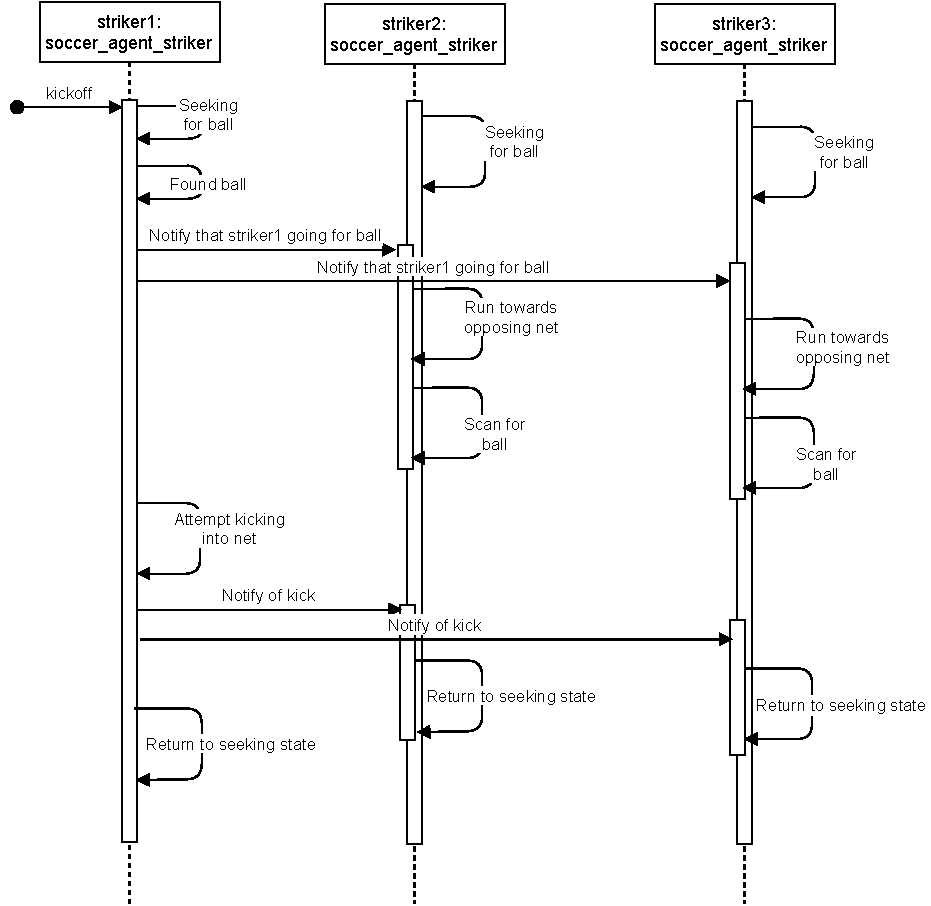
\includegraphics[scale=0.5]{fig/sequence-diagram.pdf}
	\caption{Communication between striker-type agents}
	\label{sequence-diagram}
\end{figure}

\subsubsection{Defender}
Each defender looks for its own net and runs towards it. Once there, they then defend the net by searching for the ball and, if the ball is within a certain distance of them, approaching the ball and kicking it away towards the opposing net.


\section{Implementation}
Three discrete components are involved in controlling agents: the Jason framework, the Java environment, and the Krislet player. 

\subsection{Jason}
The abstract player behaviours were first formalized in flowcharts (Figure \ref{flowchart-striker}, Figure  \ref{flowchart-defender}), and then adapted into AgentSpeak plans, which define agent actions based on their beliefs and the context they can observe. The Jason framework provides the cognitive model for executing these plans; the agent is fed percepts about the soccer simulation (such as the location of the ball, the opposing goal, etc.) and adds appropriate beliefs to its knowledge base.

\begin{figure}[]
	\centering
	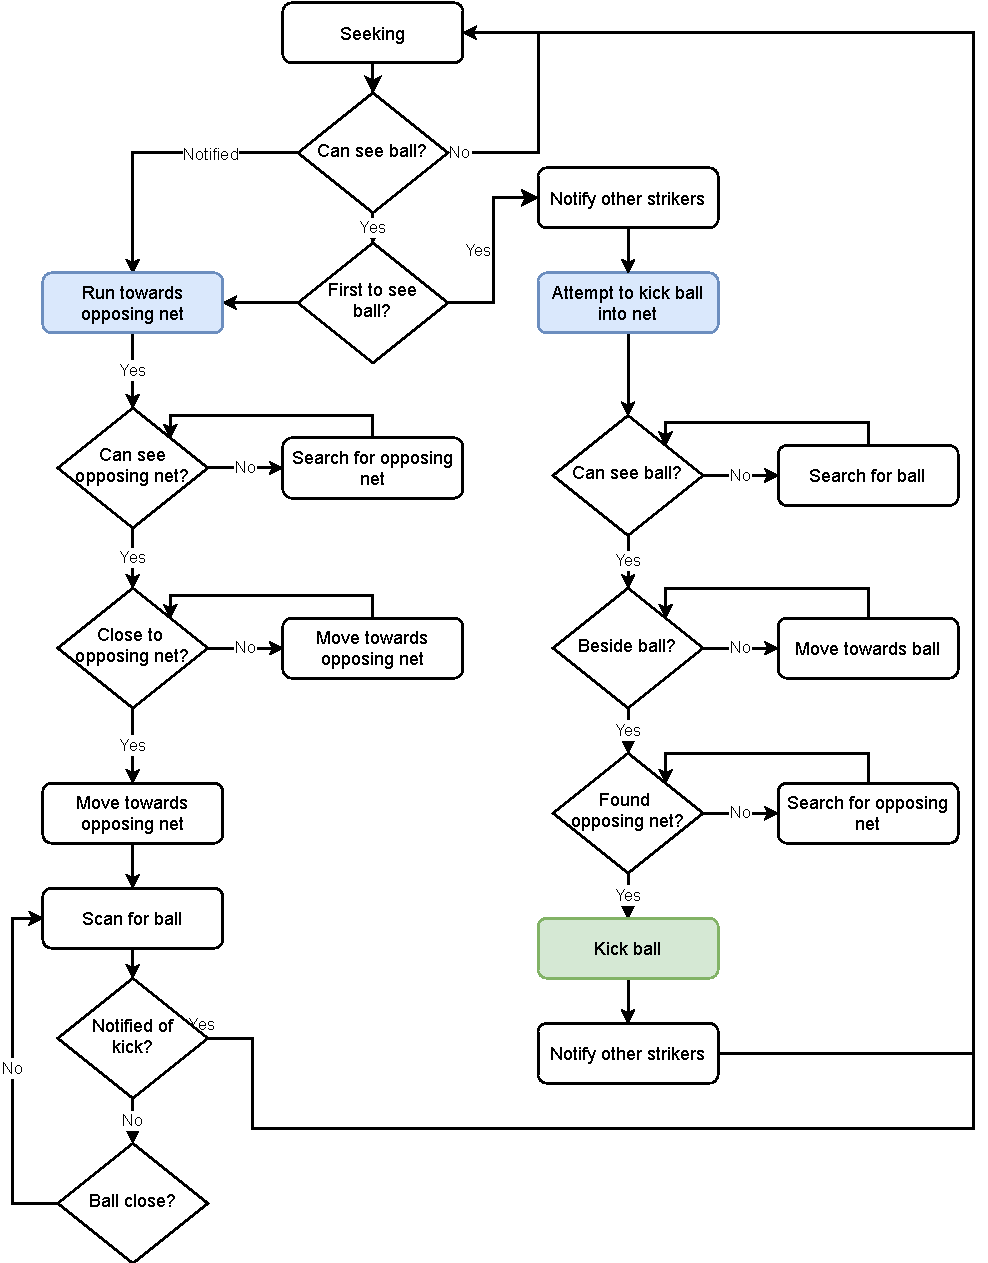
\includegraphics[scale=0.5]{fig/striker-flowchart.pdf}
	\caption{Flowchart for striker-type agents}
	\label{flowchart-striker}
\end{figure}

\begin{figure}[]
	\centering
	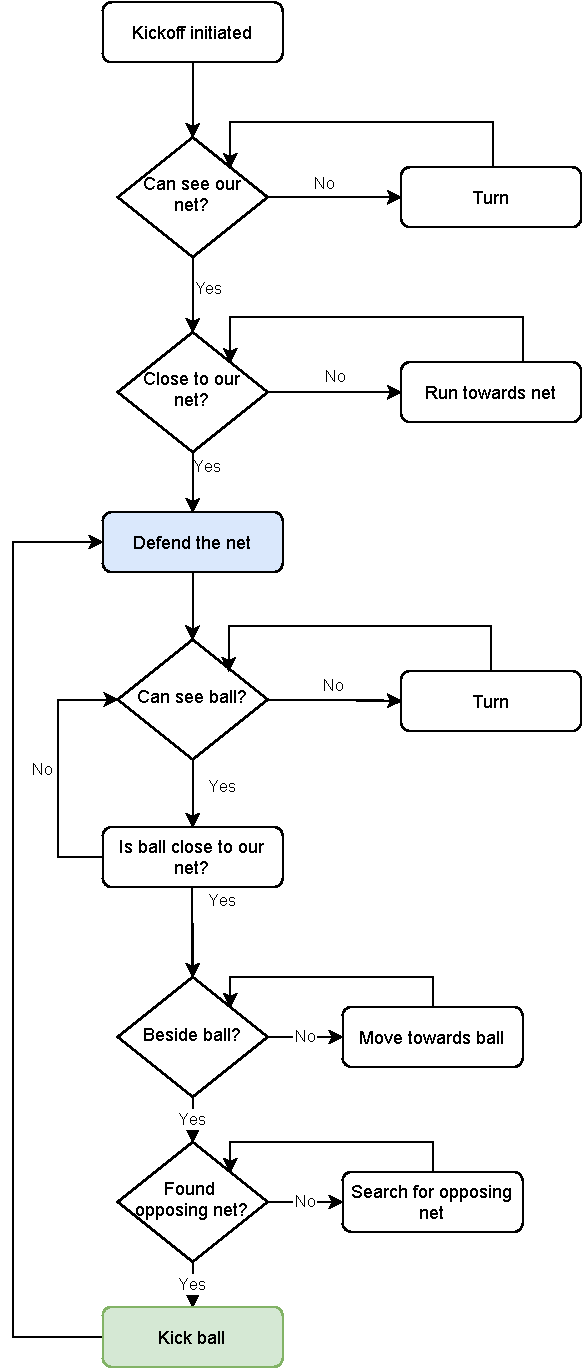
\includegraphics[scale=0.5]{fig/defender-flowchart.pdf}
	\caption{Flowchart for defender-type agents}
	\label{flowchart-defender}
\end{figure}

\subsection{Environment}
The environment is a Java class that handles the interface between the Robocup soccer environment server and the Jason framework. At program startup it initializes all Krislet objects and has callbacks to map Krislet memory objects to Jason percepts. 

\subsection{Krislet}
The Krislet program was provided as a demo agent to run in the Robocup simulation. This program was modified to be a stand alone agent for interfacing with the simulation, acting as a puppet for the Jason agent. Each Krislet object represents one Jason agent, and when created opens a socket to the soccer environment server and registers the player. Actions chosen by the Jason agent are executed by the Krislet object following the Command design pattern, which also feeds back percepts to the Jason agent.


\section{Results}
Lorem ipsum dolor sit amet, consectetur adipiscing elit. Praesent auctor, urna eu suscipit convallis, nisi urna tempus risus, eget pulvinar elit nisl ac nulla. Integer arcu augue, vehicula feugiat lobortis elementum, interdum ut augue. Nunc egestas nulla eget lorem pulvinar commodo. Nunc egestas turpis efficitur aliquet euismod. In eleifend sodales commodo. Maecenas non posuere lorem. Nullam lacus ligula, sollicitudin ac est a, congue tempor tellus. Suspendisse cursus felis fringilla, dignissim sem feugiat, pulvinar risus. Fusce nec tempus lacus. Donec ac massa at nunc pellentesque aliquet. Nam sollicitudin posuere enim, non consequat arcu cursus at. 
\section{Conclusion}
Aenean eget hendrerit nunc, vitae dapibus risus. Sed ut ultrices quam, at facilisis lectus. Fusce dapibus condimentum consectetur. Lorem ipsum dolor sit amet, consectetur adipiscing elit. Phasellus facilisis vulputate odio imperdiet condimentum. Cras accumsan nunc ac sagittis sodales. 


\section{Appendix}
\centering
\begin{figure}[h]
	\centering
	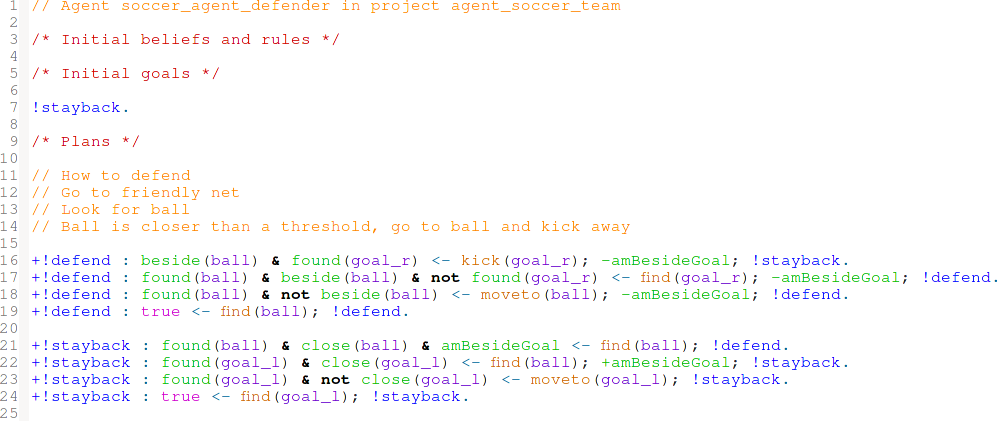
\includegraphics[width=\textwidth]{fig/defender-code.png}
	\caption{AgentSpeak code for defender-type agents}
	\label{code-defender}
\end{figure}

\begin{figure}[h]
	\centering
	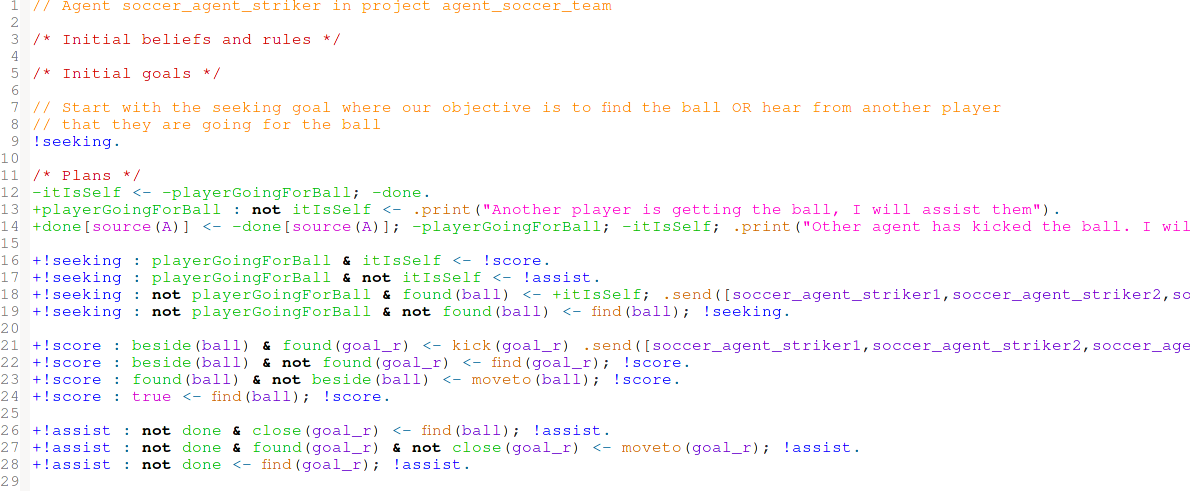
\includegraphics[width=\textwidth]{fig/striker-code.png}
	\caption{AgentSpeak code for striker-type agents}
	\label{code-striker}
\end{figure}


\end{document}
